\section{Auswertung}
\label{sec:Auswertung}
Die Werte der benutzten Schaltung sind
\begin{align*}
  L=&(10.11\pm0.03)10^{-3}\si{\henry}\\
  C=&(2.098\pm0.006)10^{-9}\si{\farad}\\
  R_1=&(48.1\pm0.1)\si{\ohm}\\
  R_2=&(509.5\pm0.5)\si{\ohm}\;.
\end{align*}
\begin{figure}
  \centering
  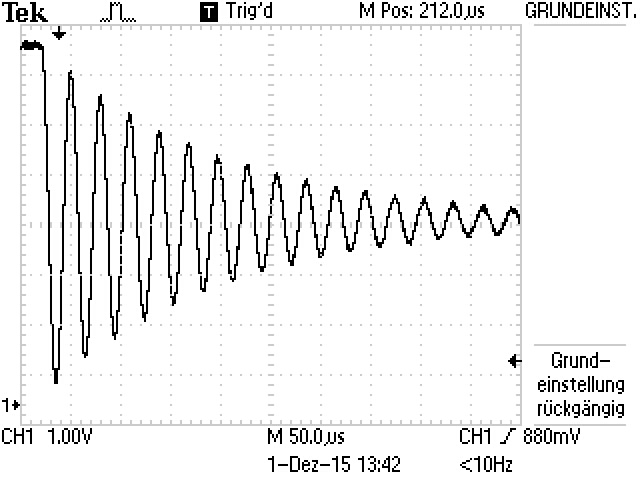
\includegraphics[width=0.78\textwidth]{Thermodruck.JPG}
  \caption{Thermodruck einer gedämpften Schwingung, aus der die Werte für
  die Tabelle \ref{fig:Messwertegedaempfteschwingung}, sowie für die Ausgleichsrechnung
  nach Gleichung \eqref{eqn:loesung} für die Berechnung von $R_{eff}$ und $T_{ex}$
  stammen. Die roteingezeichneten Linien sind die Begrenzenden Funktionen.}
  \label{fig:termodruck}
\end{figure}
In der Tabelle \ref{fig:Messwertegedaempfteschwingung} werden die
abgelesenden Werte aus Abbildung \ref{fig:termodruck}
aufgeführt. Die Ausgleichsrechnung nach Gleichung
\eqref{eqn:gedaempfte_schwingung} hat die Form $A\symup{exp}(Bt)\symup{cos}(Ct+D)+E$
und die Fitparameter
\begin{align*}
  A&=A_0=-4.4\pm0.1  \\
  B&=-2\pi\mu=0(-5.5\pm0.2)10^3  \\
  C&=-2\pi\nu=(2.099\pm0.003)10^5   \\
  D&=\eta=-6.90\pm0.06  \\
  E&=7.4\pm1.2)10^{-2}\;.
\end{align*}
Der Fitparameter $E$ wurde hinzugefügt, da es eine Offsetspannung gibt.
Der effektive Widerstand $R_{eff}$ ist nach Gleichung \eqref{eqn:breite_resonanzkurve}
 zu berechnen und
die Abklingdauer $T_{ex}$ nach Gleichung \eqref{eqn:abklingzeit}. Die berechneten
Werte sind
\begin{align*}
    R_{eff}=&111.9\pm3.3\si{\ohm}\\
    T_{ex}=&(1.81\pm0.05)10^{-4}\si{\second}\;.
\end{align*}
Die Werte weichen von dem verbauten Widerstand $R_1=48.1\si{\ohm}$ um $63.8\si{\ohm}$
ab. Dies lässt sich durch den Innenwiderstand des Generator von $50\si{\ohm}$ erklären.
In den folgenden Berechnungen wird dieser Innenwiderstand mitbetrachtet.
\begin{table}
  \centering
  \begin{tabular}{c c}
    \toprule
    Zeit in $\si{\micro\second}$ & Spannung in $\si{\volt}$  \\
    \midrule
     35  &  -3.2  \\
     50  &   3.1  \\
     65  &  -2.7  \\
     80  &   2.6  \\
     95  &  -2.3  \\
    110  &   2.1  \\
    125  &  -1.9  \\
    140  &   1.9  \\
    150  &  -1.6  \\
    165  &   1.6  \\
    180  &  -1.3  \\
    195  &   1.4  \\
    210  &  -1.1  \\
    225  &   1.2  \\
    240  &  -0.9  \\
    255  &   1.0  \\
    270  &  -0.9  \\
    285  &   0.9  \\
    300  &  -0.6  \\
    315  &   0.8  \\
    \bottomrule
  \end{tabular}
  \caption{In der Tabelle sind die aus dem Thermodruck Abgelesenden Werte abgebildet.
           Es sind die ersten $20$ Extrema der Schwingungskurve. Die Zeit ist
            in  $\si{\micro\second}$ angegeben und die Spannung in $\si{\volt}$.
            Bei der Spannung liegt ein Fehler von $0.1\si{\volt}$ und ber der Zeit
            ein Fehler von $0.1\si{\micro\second}$ vor. Die Werte werden für die
            Ausgleichsrechnung in \ref{fig:gedaempfteschwingung} verwendet.}
  \label{fig:Messwertegedaempfteschwingung}
\end{table}
Der experimentell bestimmte Widerstandswert für den aperiodischen Grenzfall
und  der nach Gleichung \eqref{eqn:bedingung-ap-grenzfall} sind
\begin{align*}
  R_{ap_e}=&(3350\pm10)\si{\ohm}\\
  R_{ap_t}=&(4390\pm9.0)\si{\ohm}\\
  \text{Relativer Fehler}\\
   &24.8\%\;.
\end{align*}


In Abbildung \ref{fig:Kondensatorspannung} sind die
Messwerte zu der Frequenzabhängigkeit der Kondensatorspannung in Abhängigkeit
von der Frequenz dargestellt. In Abbildung \ref{fig:Resonanzkurve} ist die
Resonanzkurve mit linear skalierter x-Achse dargestellt. Die aus der Abbildung
\ref{fig:Kondensatorspannung}
entnommende Frequenz bei der der Phasenwinke $\phi=90°$ ist und die
nach $\omega_0=\sqrt{\frac{1}{CL}}$ errechnete sind
\begin{align*}
\omega_{0_e}=&(33500.0\pm0.1)\si{\hertz}\\
\omega_{0_t}=&(2.171\pm0.004)10^5\si{\hertz}\\
\text{Relativer Fehler}\\
 &84.6\%\;.
\end{align*}
 Die Breite der
Resonanzkurve $\omega_+-\omega_- $, ist nach Gleichung \eqref{}
 und experimentell bestimmt
\begin{align*}
 \omega_{+_t}-\omega_{-_t}=&(5.04\pm0.016)10^4\si{\hertz}\\
 \omega_{+_e}-\omega_{-_e}=&(10000.0\pm0.1)\si{\hertz}\\
 \text{Relativer Fehler}\\
  &80.1\%\;.
\end{align*}
Für den experimentell bestimmten Wert von $\omega_{+_e}-\omega_{-_e}$ wurden
die Frequenzen $28000.0\si{\hertz}$ und $38000.0\si{\hertz}$ verwendet.
Die Güte der Resonanzkurve ist nach Gleichung \eqref{eqn:guete}
\begin{align*}
  q_t=&3.923\pm0.009\\
  q_e=&3.35\pm0.000035\\
  \text{Relativer Fehler}
  14.6\%\;.
\end{align*}
\begin{figure}
  \centering
  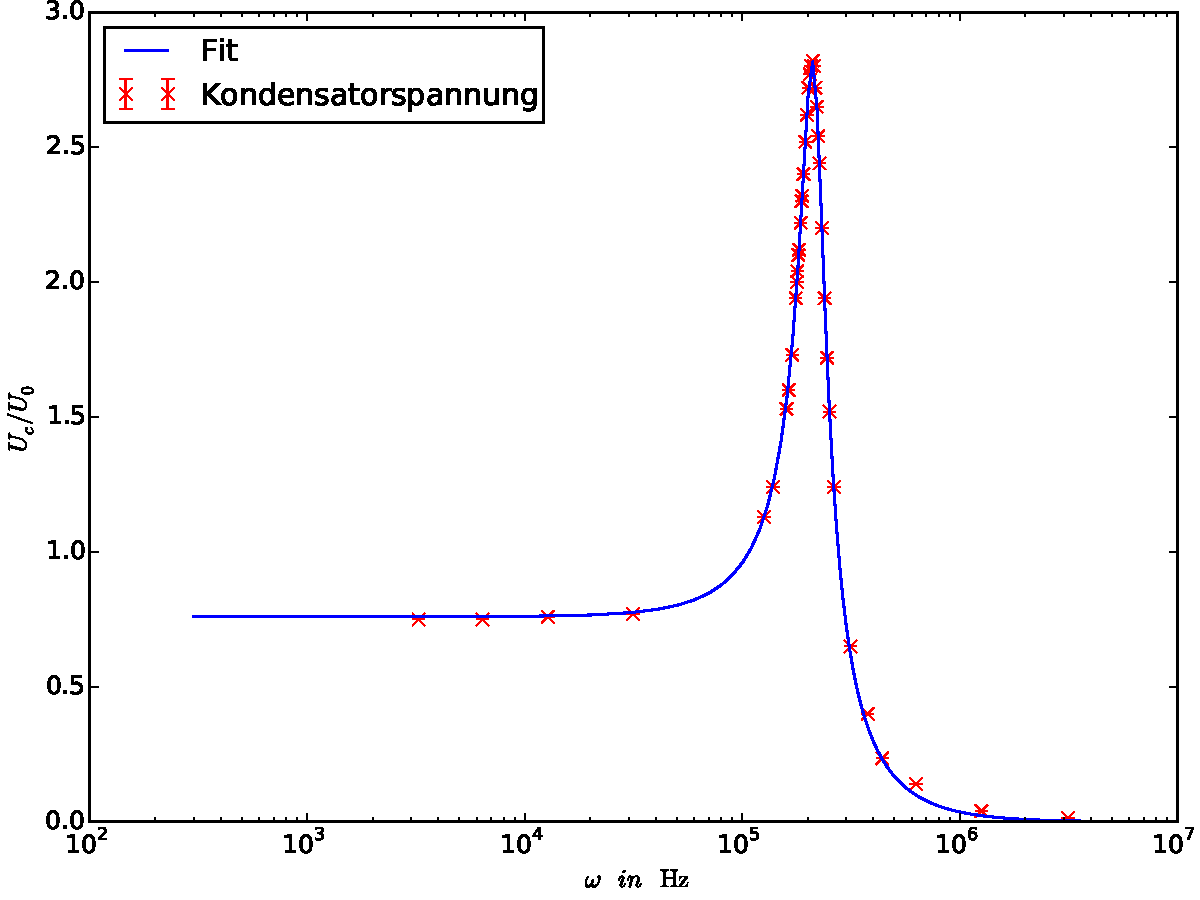
\includegraphics[width=0.78\textwidth]{Kondensatorspannung.pdf}
  \caption{Abbildung der in \ref{fig:Messwerte} aufgeführten Messwerte.
  Die normierte Kondensatorspannung $U_c/U$ wird in Abhängigkeit von der
  Frequenz dargestellt.}
  \label{fig:Kondensatorspannung}
\end{figure}
\begin{figure}
  \centering
  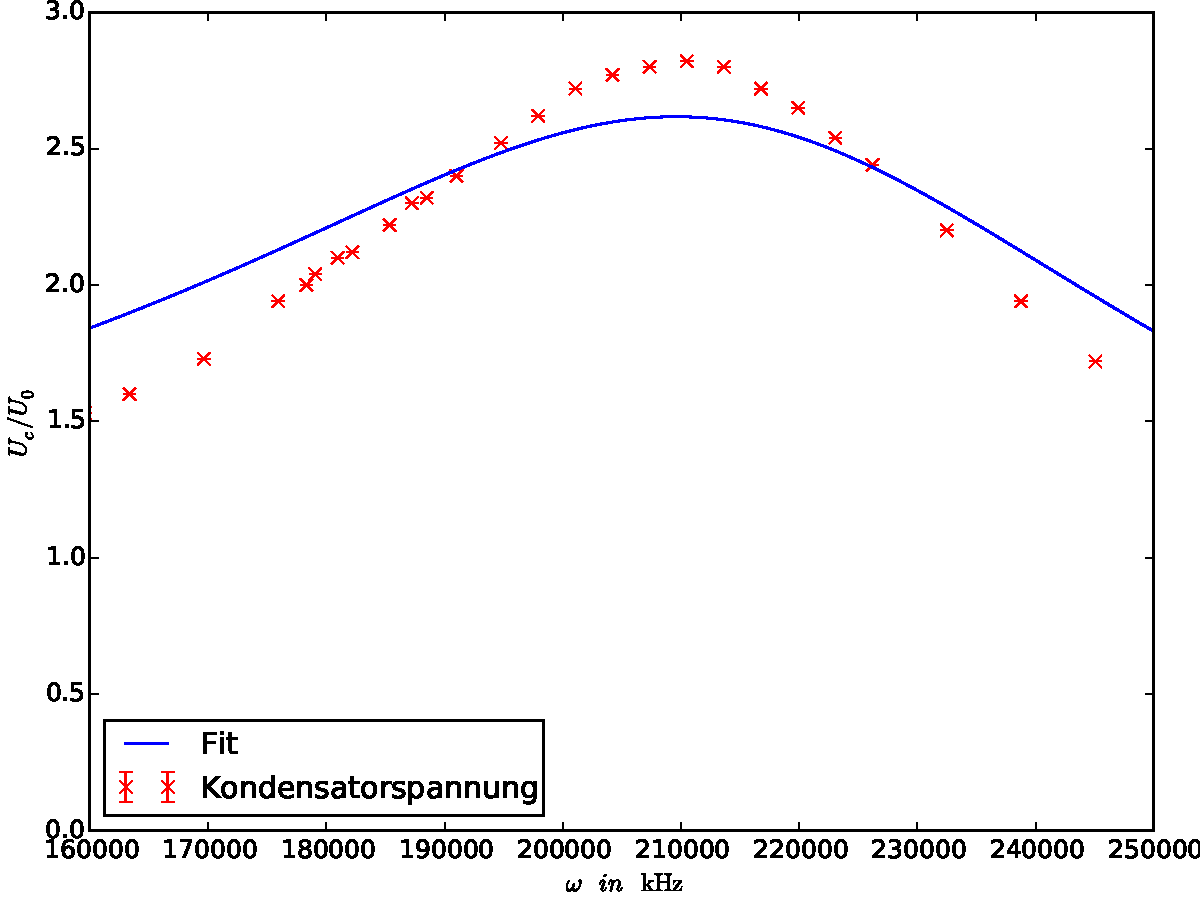
\includegraphics[width=0.78\textwidth]{Resonanzkurve.pdf}
  \caption{Abbildung von Messwerten in der Nähe von der Phasenverschiebung $\phi=90°$.
  In ihr ist die Resonanzkurve zu sehen. Die normierte Kondensatorspannung $U_c=U$
  ist in abhängigkeit von der Frequenz aufgetragen.}
  \label{fig:Resonanzkurve}
\end{figure}
Mit den Messwerten in der Tabelle \ref{fig:Messwerte} sind die  Abbildungen
\ref{fig:Kondensatorspannung}, \ref{fig:Resonanzkurve},
\ref{fig:phasenverschiebung} und \ref{fig:linphasenverschiebung}
entstanden.
\begin{table}
  \centering
  \begin{tabular}{c c c}
    \toprule
    \omega/$\si{\hertz}$ & $U/U_c$ & $a/\si{\micro\second}$ \\
    \midrule
         517.2  &  0.750  &  0     \\
        1017.0  &  0.750  &  0     \\
        2031.0  &  0.760  &  0     \\
        5000.0  &  0.770  &  0     \\
       10000.0  &  0.850  &  1,50  \\
       20000.0  &  1.130  &  1.56  \\
       22000.0  &  1.240  &  1.80  \\
       25400.0  &  1.530  &  2.60  \\
       26000.0  &  1.600  &  2.60  \\
       27000.0  &  1.730  &  2.80  \\
       28000.0  &  1.940  &  3.20  \\
       28380.0  &  2.000  &  3.60  \\
       28500.0  &  2.040  &  3.60  \\
       28800.0  &  2.100  &  4.00  \\
       29000.0  &  2.120  &  3.80  \\
       29500.0  &  2.220  &  3.90  \\
       29800.0  &  2.300  &  3.80  \\
       30000.0  &  2.320  &  4.00  \\
       30400.0  &  2.400  &  4.20  \\
       31000.0  &  2.520  &  4.60  \\
       31500.0  &  2.620  &  5.20  \\
       32000.0  &  2.720  &  5.60  \\
       32500.0  &  2.770  &  6.00  \\
       33000.0  &  2.800  &  6.20  \\
       33500.0  &  2.820  &  7.00  \\
       34000.0  &  2.800  &  7.60  \\
       34500.0  &  2.720  &  7.80  \\
       35000.0  &  2.650  &  8.20  \\
       35500.0  &  2.540  &  8.40  \\
       36000.0  &  2.440  &  8.80  \\
       37000.0  &  2.200  &  9.40  \\
       38000.0  &  1.940  &  9.20  \\
       39000.0  &  1.720  &  9.20  \\
       40000.0  &  1.520  & 10.20  \\
       42000.0  &  1.240  & 10.00  \\
       50000.0  &  0.650  &  9.20  \\
       60000.0  &  0.400  &  8.00  \\
       70000.0  &  0.235  &  7.00  \\
      100000.0  &  0.140  &  4.80  \\
      200000.0  &  0.040  &  2.20  \\
      500000.0  &  0.015  &        \\
  \end{tabular}
  \caption{In der Tabelle sind die Frequenz $\omega$in $\si{\hertz}$, die normierte
  Kondensatorspannung und der Abstand der Nulldurchgänge $a$ in $\si{\micro\second}$
   angegeben. Die Fehler sind $\pm0.1\si{\hertz}$,$ \pm0.001$ und
   $\pm0.01\si{\micro\second}$.}

  \label{fig:Messwerte}
\end{table}
In der Abblidung \ref{fig:phasenverschiebung} ist der Phasenwinkel $\phi$ in Abhängingkeit
von der Frequenz dargestellt und der Bereich um $\phi=90°$ nocheinmal mit
linear skalierter x-Achse in Abbildung \ref{fig:linphasenverschiebung} . Die
Frequenzen $\omega_{1}$ und
$\omega_{2}$  sind nach Gleichung \eqref{} und experimenteller Bestimmung
\begin{align*}
  \omega_{1_t}=&( 2.466\pm0.005)10^5\si{\hertz}\\
  \omega_{2_t}=&(1.934\pm0.004)10^5\si{\hertz}\\
  \omega_{1_e}=&2.98 \cdot10^4\si{\hertz}\\
  \omega_{2_e}=&3.9 \cdot10^4\si{\hertz}\\
  \text{Relativer Fehler}\\
   &87.8\%\\
   &79.8\%\;.
\end{align*}
Die Resonanzfrequenz wird bestimmt durch Gleichung \eqref{eqn:resonanzfrequenz}.
Der berechnete und der im Experiment bestimmte Wert sind
\begin{align*}
\omega_{res_t}=&(2.171\pm0.004)10^5\si{\hertz}\\
\omega_{res_e}=&(3.4\pm0.01)10^4\si{\hertz}\\
\text{Relativer Fehler}\\
84.3\%\;.
\end{align*}
\begin{figure}
  \centering
  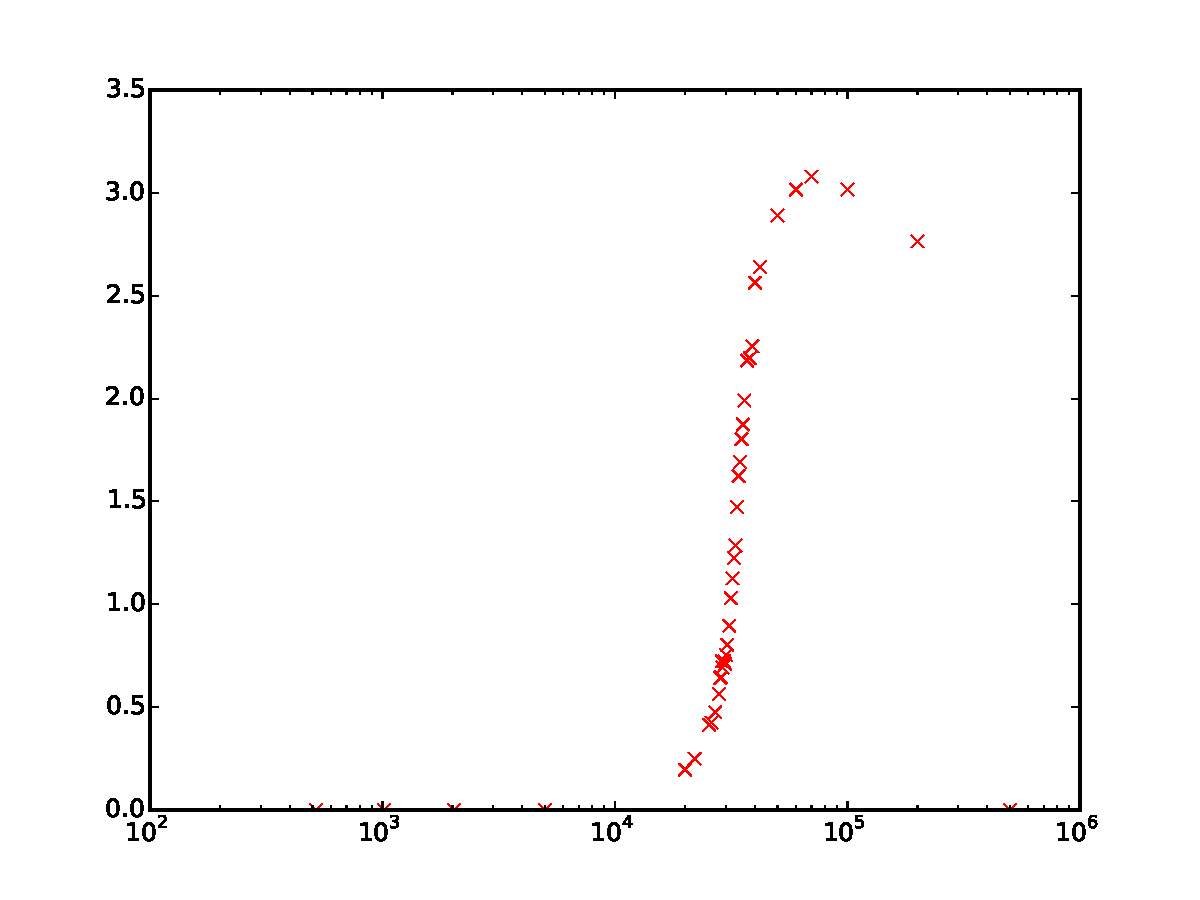
\includegraphics[width=0.78\textwidth]{phasenverschiebung.pdf}
  \caption{Abbildung der Phasenwinkel der Messwerte von Tabelle \ref{fig:Messwerte} in
  abhängigkeit von der Frequenz dargestellt werden. Der zu erwartende Verlauf ist
  ein Arkustangens.}
  \label{fig:phasenverschiebung}
\end{figure}
\begin{figure}
  \centering
  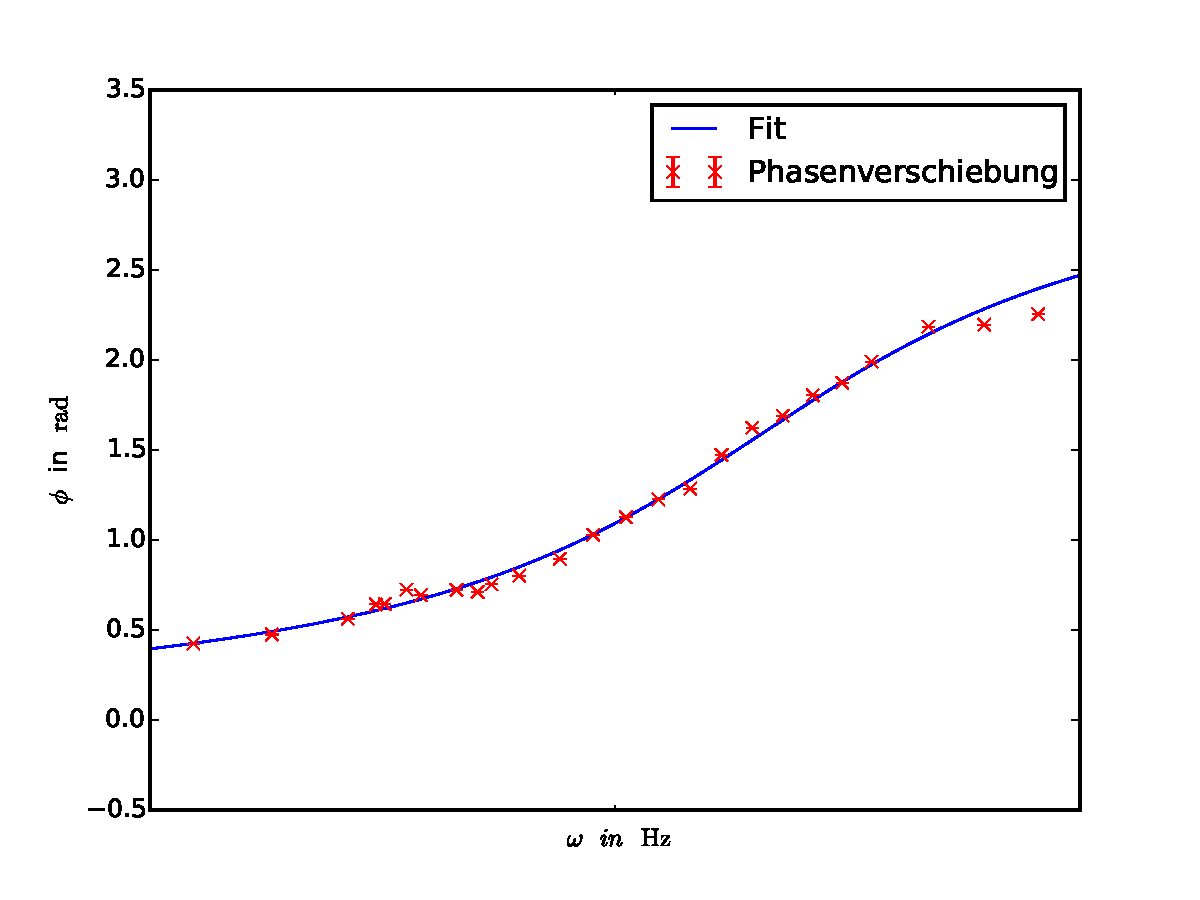
\includegraphics[width=0.78\textwidth]{linphasenverschiebung.pdf}
  \caption{Abbildung von Messwerten in der Nähe von der Phasenverschiebung $\phi=90°$.
          Der Phasenwinkel $\phi$ ist in abhängigkeit von der Frequenz gegeben.}
  \label{fig:linphasenverschiebung}
\end{figure}
